\documentclass{article}

\IfFileExists{tmlr.sty}{%
  \usepackage{tmlr}
}{%
  \usepackage[margin=1in]{geometry}
  \usepackage{natbib}
  \bibliographystyle{abbrvnat}
}

\usepackage{amsmath,amssymb,amsthm}
\usepackage{graphicx}
\usepackage{booktabs}
\usepackage{hyperref}
\usepackage{microtype}
\usepackage{xcolor}
\usepackage{algorithm}
\usepackage{algpseudocode}
\usepackage{mathtools}
\usepackage{enumitem}
\usepackage{multirow}
\usepackage{tikz}
\usepackage{pgfplots}
\pgfplotsset{compat=1.17}
\usetikzlibrary{arrows.meta,positioning,shapes.geometric,fit,backgrounds,calc}

\hypersetup{colorlinks=true,linkcolor=blue,citecolor=blue,urlcolor=blue}

\newtheorem{theorem}{Theorem}
\newtheorem{corollary}[theorem]{Corollary}
\newtheorem{proposition}[theorem]{Proposition}
\newtheorem{lemma}[theorem]{Lemma}
\newtheorem{definition}{Definition}
\newtheorem{remark}{Remark}
\newtheorem{assumption}{Assumption}

\title{PAVO: Pipeline-Aware Voice Orchestration with\\Demand-Conditioned Inference Routing}

% Author information hidden for double-blind review

\begin{document}

\maketitle

\begin{abstract}
Voice agents built on ASR-LLM-TTS pipelines allocate compute statically, ignoring per-turn variation in complexity and hardware state. We introduce PAVO (Pipeline-Aware Voice Orchestrator), which treats the three-stage pipeline as a jointly optimizable inference graph with demand-conditioned routing. The core contribution is an empirical characterization of \emph{inter-stage coupling constraints}---quality dependencies where upstream ASR configuration bounds feasible downstream LLM options---validated on $n=3{,}630$ direct calibration measurements across two hardware platforms (H100, M3) and two LLM families. Direct inference experiments on NVIDIA H100 with Whisper, Llama~3.1 8B, and Gemma2~2B show 12\% lower P95 latency than fixed cloud ($p = 2\times10^{-6}$), with coupling binding across all 21 noise conditions. Routing simulation on the synthetic PAVO-Bench (50K turns, five complexity levels, $\kappa=0.81$), parameterized by these measured latencies, shows 34\% lower median latency and 71\% lower energy versus fixed-cloud at 1.6\,pp BERTScore cost. An 85K-parameter MLP meta-controller trained via multi-objective PPO (100K steps on H100, 106\,s wall-clock) reduces coherence failure rate by 7.9$\times$ versus unconstrained routing. Code and data are publicly available.\footnote{\url{https://anonymous.4open.science/r/pavo-bench}}
\end{abstract}

% ============================================================================
\section{Introduction}
\label{sec:intro}

Voice interfaces built on large language models now handle open-ended reasoning, multi-turn dialogue, and tool use~\citep{openai2024gpt4o,dubey2024llama3,team2024gemma2}. The infrastructure underpinning these systems has not kept pace: nearly every deployed voice agent runs a fixed ASR$\to$LLM$\to$TTS pipeline at a predetermined precision and hardware tier, regardless of what each turn actually requires~\citep{oord2016wavenet,ren2021fastspeech,kim2021vits,dettmers2022llmint8,frantar2022gptq,lin2024awq}.

The resulting waste is quantifiable. Llama~3.1 8B on A100 at batch size 1 requires $\sim$500\,ms TTFT and $\sim$30\,ms per output token~\citep{mlperf2025}, placing an 80-token voice response at 2{,}900\,ms. A date-lookup query needs neither an 8B model nor cloud compute; Gemma~2B on-device answers it in under 1{,}000\,ms. Fixed pipelines cannot exploit this disparity. A less obvious failure mode runs the other direction: Gemma~4B INT8 on Jetson achieves 4--6 tokens/second~\citep{song2023powerinfer}, requiring 13--20 seconds for 80-token responses. For complex queries, fixed-edge deployment is \emph{slower} than cloud. Neither fixed-cloud nor fixed-edge is universally optimal; the right strategy depends on per-turn complexity.

\paragraph{Why this problem matters at scale.} Voice assistants serve billions of daily queries~\citep{openai2024gpt4o}. At this scale, a 12\% P95 latency reduction eliminates millions of SLO violations per day; a 71\% energy reduction translates to measurable data center power savings. Current production systems (Alexa, Google Assistant, Siri) use fixed pipelines because no operational framework exists for enforcing quality constraints across pipeline stages during routing. PAVO provides this framework. The target deployment is enterprise voice infrastructure where modular ASR-LLM-TTS pipelines are operationally mandated for transcript logging, privacy compliance, and cost control.

Two properties of voice pipelines motivate PAVO. First, stage outputs depend on input quality: ASR errors propagate to the LLM, creating dependencies that make per-stage optimization non-separable. We characterize these as coupling constraints and enforce them during routing. Second, turn complexity is partially predictable from pre-transcription acoustic features before the LLM stage begins, so a proactive controller conditioned on these features reduces coherence failures 3.1$\times$ versus reactive policies (Table~\ref{tab:ablation_routing}). Benchmark simulation results are corroborated by direct inference experiments on NVIDIA H100 GPU running Whisper, Llama~3.1 8B, and Gemma2~2B across 21 noise conditions.

\paragraph{Contributions.}
\begin{enumerate}[leftmargin=*,itemsep=2pt]
\item \textbf{Inter-stage coupling constraints as an operational routing framework.} To our knowledge, the first empirical characterization of quality dependencies between ASR, LLM, and TTS pipeline stages, operationalized as hard constraints during inference routing. Enforcement reduces coherence failure rate from 7.1\% to 0.9\% on the 50K-turn benchmark (7.9$\times$) and eliminates 495 violations per 1{,}000 turns on real H100 hardware, at a measured cost of 110\,ms median latency (Table~\ref{tab:ablation_coupling}).

\item \textbf{Demand-conditioned multi-objective routing via RL.} A deployable 85K-parameter MLP meta-controller (0.3\,ms inference on Cortex-A78) trained via multi-objective PPO, conditioned on a 12-dimensional demand vector with four pre-transcription acoustic features. On H100, the policy compresses P95 tail latency by 167\,ms versus fixed-cloud with statistical significance across 5 seeds (Section~\ref{sec:gpu}); the full benchmark evaluation shows 34\% median-latency and 71\% energy reductions.

\item \textbf{PAVO-Bench and two-tier evaluation.} A 50{,}000-turn synthetic benchmark (40K/10K split, $\kappa=0.81$) generated on H100 GPU, evaluated at two tiers: (a)~direct inference experiments on Lambda Labs H100 with real Whisper/Llama/Gemma models covering E2E latency (200 samples), 21 noise conditions, cross-dataset generalization (LibriSpeech + FLEURS), and model scaling; and (b)~routing simulation across 9 baselines and 50K turns, parameterized by the measured latencies.
\end{enumerate}

% ============================================================================
\section{Related work}
\label{sec:related}

\paragraph{Voice pipeline architectures.} Three generations of voice agents differ in where intelligence sits: finite-state NLU~\citep{stivers2009universals,young2013pomdp}, neural speech-text models~\citep{rubenstein2023audiopalm}, and LLM-centric cascades~\citep{defossez2024moshi,xie2024miniomni} or end-to-end audio models~\citep{openai2024gpt4o}. End-to-end models eliminate inter-stage latency but sacrifice five properties that enterprise deployments require: (1)~\emph{transcript logging}---regulatory compliance (HIPAA, GDPR) mandates storing verbatim transcripts, which end-to-end audio-to-audio models do not produce; (2)~\emph{per-stage hardware placement}---modular pipelines can run ASR on-device for privacy while routing LLM to cloud for capability, a split impossible with monolithic models; (3)~\emph{component upgradeability}---replacing one ASR or TTS model without retraining the entire system; (4)~\emph{cost control}---per-stage metering enables fine-grained billing; and (5)~\emph{interpretability}---intermediate transcripts enable debugging and quality auditing. These constraints explain why all major deployed voice assistants (Alexa, Google Assistant, Siri) use modular pipelines despite the availability of end-to-end alternatives. Prior work on ASR error propagation in dialogue~\citep{errattahi2018asr} establishes that transcription quality has outsized downstream impact---motivating our coupling characterization.

\paragraph{Mixture-of-experts and adaptive inference.} MoE routing~\citep{shazeer2017moe,jacobs1991mixture} blends expert outputs for a single model stage. Adaptive inference systems~\citep{snell2024scaling} cascade between model tiers within a single stage. Both operate on \emph{one stage in isolation}: MoE blends Gemma and Llama outputs for the LLM stage; cascaded routing runs a small model first and escalates if quality is insufficient. Neither considers that the LLM routing decision depends on ASR output quality, which depends on the ASR configuration chosen. PAVO makes a \emph{joint three-stage decision} (one per pipeline stage per turn) subject to cross-stage coupling constraints---a structurally different optimization problem.

\paragraph{Inference serving.} Clipper~\citep{clipper2017} introduced per-query model selection for latency SLOs. INFaaS~\citep{romero2021infaas} adds cost-aware variant selection. Shepherd~\citep{gujarati2023shepherd} applies RL-based routing between model tiers. \citet{alizadeh2024llmflash} demonstrate efficient LLM inference on memory-constrained devices but use a single fixed configuration. \citet{song2023powerinfer} exploit neuron activation locality for fast consumer-GPU inference but do not consider multi-stage pipeline routing. None of these systems model inter-stage quality propagation or enforce coupling constraints during routing.

\paragraph{What PAVO adds.} Table~\ref{tab:comparison} summarizes. The gap PAVO fills is specific: prior routing systems optimize a single inference stage and assume stage quality is independent of upstream configuration. This assumption fails in voice pipelines, where a low-quality ASR transcript degrades LLM output.

\begin{table}[t]
\centering
\caption{Comparison with related systems.}
\label{tab:comparison}
\small
\begin{tabular}{lccccc}
\toprule
System & Pipeline & Multi-tier & Feedback & Voice & Coupling \\
 & aware & routing & loop & specific & constrs \\
\midrule
Clipper~\citep{clipper2017}          & No   & Yes & No  & No   & No  \\
INFaaS~\citep{romero2021infaas}      & No   & Yes & No  & No   & No  \\
Shepherd~\citep{gujarati2023shepherd}& No   & Yes & Yes & No   & No  \\
Hybrid LLM~\citep{snell2024scaling}  & No   & Yes & No  & No   & No  \\
\citet{alizadeh2024llmflash}         & No   & Yes & No  & No   & No  \\
Moshi~\citep{defossez2024moshi}      & Part.$^\dagger$& No  & No  & Yes  & No  \\
\textbf{PAVO (ours)}               & \textbf{Yes} & \textbf{Yes} & \textbf{Yes} & \textbf{Yes} & \textbf{Yes} \\
\bottomrule
\end{tabular}
\vspace{2pt}\\
{\scriptsize $^\dagger$Moshi uses an internal audio-codec$\to$LM$\to$codec structure but operates end-to-end; stages are not independently configurable.}
\end{table}

% ============================================================================
\section{Problem formulation}
\label{sec:formulation}

\subsection{Voice pipeline as a compute graph}

Let the voice pipeline be a DAG $\mathcal{G}=(\mathcal{V},\mathcal{E})$ with $\mathcal{V}=\{\text{ASR},\text{LLM},\text{TTS}\}$ and $\mathcal{E}=\{(\text{ASR},\text{LLM}),(\text{LLM},\text{TTS})\}$. Each stage $v_i$ has a finite configuration set $\mathcal{C}_i$; each $c_{i,j}\in\mathcal{C}_i$ is a tuple $(m_{i,j}, q_{i,j}, h_{i,j}, \beta_{i,j})$ specifying model variant, quantization level $q\in\{\text{FP16},\text{INT8},\text{INT4}\}$~\citep{jacob2018quantization,frantar2022gptq,lin2024awq}, hardware placement $h\in\{\text{cloud},\text{edge},\text{on-device}\}$, and batch size. The joint configuration space is $\mathcal{C}=\mathcal{C}_1\times\mathcal{C}_2\times\mathcal{C}_3$.

For dialogue turn $t$ with input audio $x_t$ and conversation history $z_t$, configuration $c\in\mathcal{C}$ induces four measurable outcomes:
\begin{align}
L(c,x_t,z_t) &\in \mathbb{R}_{\geq 0} \;\;\text{(end-to-end latency, ms)} \label{eq:L}\\
E(c,x_t,z_t) &\in \mathbb{R}_{\geq 0} \;\;\text{(energy, J)} \label{eq:E}\\
M(c,x_t,z_t) &\in [0,1] \;\;\;\;\text{(peak memory fraction)} \label{eq:M}\\
Q(c,x_t,z_t) &\in [0,1] \;\;\;\;\text{(composite quality)} \label{eq:Q}
\end{align}
Quality $Q = 0.4\cdot(1-\text{WER}) + 0.4\cdot\text{BERTScore} + 0.2\cdot\text{UTMOS}_{\text{norm}}$, with weights from grid search on 200 held-out turns maximizing MOS correlation~\citep{ribeiro2011crowdmos,saeki2022utmos,zhang2020bertscore} ($r=0.74$).

\subsection{Routing optimization}

Given demand distribution $\mathcal{P}(x,z)$ and operator weights $(w_L,w_E,w_M,w_Q)$ with $\sum_k w_k=1$, we seek policy $\pi:\mathcal{S}\to\mathcal{C}$ minimizing:
\begin{equation}
J(\pi) = \mathbb{E}_{(x,z)\sim\mathcal{P}}\bigl[w_L\hat{L} + w_E\hat{E} + w_M\hat{M} - w_QQ\bigr]
\label{eq:objective}
\end{equation}
where $\hat{L}=L/L_{\text{ref}}$, $\hat{E}=E/E_{\text{ref}}$, $\hat{M}=M/M_{\text{ref}}$ are normalized against Fixed-Cloud references. System state $s_t=[a_t,h_t,n_t,d_t]\in\mathbb{R}^{12}$ is defined in Section~\ref{sec:signal}.

\subsection{ASR--LLM coupling: task-dependent error propagation}
\label{sec:coupling}

\begin{definition}[Stage quality threshold]
For stage $v_j$ with configuration $c_j$, the quality threshold $\theta_j(c_j)\in[0,1]$ is the minimum output quality required from the preceding stage for $v_j$ to produce acceptable output (BERTScore~\citep{zhang2020bertscore,devlin2019bert} $\geq 0.80$, UTMOS $\geq 3.50$).
\end{definition}

The coupling constraint between connected stages is:
\begin{equation}
Q_i(c_i,u_i) \geq \theta_j(c_j) \quad \forall\,(v_i,v_j)\in\mathcal{E}
\label{eq:coupling}
\end{equation}

The central empirical finding of our coupling analysis is that ASR errors propagate to downstream LLM quality in a \emph{regime-dependent} manner: factual tasks exhibit a sharp accuracy cliff at low word-error rates, while semantic tasks degrade gracefully across a wide WER range. This two-regime structure governs the design of PAVO's quality constraint and explains why a single conservative threshold is both necessary and sufficient for pipeline routing.

\paragraph{Regime 1: Factual coupling (sharp cliff).}
We calibrated the coupling threshold on two independent hardware platforms. On Apple M3, 30 factual QA pairs evaluated at 2\% WER increments (Table~\ref{tab:coupling_measured}) show exact-match accuracy on Llama~3.1 8B dropping 34\,pp at $\theta = 2\%$ WER (from 0.97 to 0.63; Fisher exact $p = 0.038$; Clopper--Pearson 95\% CI $[0.44, 0.80]$). On H100, a larger-scale calibration with $n=200$ queries at each of 9 WER levels for two models ($n_{\text{total}} = 3{,}600$ LLM calls; Table~\ref{tab:gpu_coupling}) reveals model-dependent coupling structure: Gemma2~2B shows a sharp cliff at WER $= 1\%$ (exact-match drops from 0.825 to 0.680, then to 0.585 at 2\%), while Llama~3.1 8B degrades more gradually (0.925 to 0.785 at 1\%, stabilizing around 0.71--0.73 for higher WERs). The combined direct calibration evidence spans $n = 3{,}630$ measurements across two hardware platforms and two LLM families. The cliff-like profile is consistent with factual queries' reliance on verbatim named entities and numerical values, where a single substitution error can alter the answer. The model-size dependence---smaller models are more sensitive to upstream errors---implies that coupling thresholds should be calibrated per LLM. This regime applies to PAVO-Bench complexity levels L1--L2 (factual retrieval and single-step reasoning), which constitute 55\% of turns.

\paragraph{Regime 2: Semantic coupling (graceful degradation).}
On the H100 GPU, the quality score for Llama~3.1 8B remains between 0.789 and 0.948 across all WER levels (Table~\ref{tab:gpu_coupling}), indicating gradual degradation rather than a sharp cliff for larger models. For Gemma2~2B, quality degrades more steeply but stabilizes: quality at WER~$\geq 5\%$ fluctuates between 0.740 and 0.796, compared to the 0.875 baseline. The contrast between exact-match and quality score is instructive: at 10\% WER, Llama's exact-match has fallen from 0.925 to 0.700, but its quality score remains at 0.789---semantic matching tolerates moderate transcription noise. This regime applies to L3--L5 (open-ended, emotional, tool-use queries).

\paragraph{Operational threshold.}
PAVO adopts a uniform quality threshold $\theta = 2\%$ WER. This choice is conservative by design. At inference time, the router must commit to a pipeline configuration \emph{before} ASR completes and before the downstream task complexity is known. A task-adaptive threshold $\theta(k)$ per complexity level $k$ would require either a preliminary ASR pass (doubling latency) or an oracle for query type (unavailable in streaming settings). The uniform $\theta = 2\%$ therefore functions as a worst-case guarantee: it satisfies the binding constraint for factual queries while remaining well within the safe region for semantic queries. The cost of this conservatism is a median latency overhead of 110\,ms ($+3.7\%$ relative to the unconstrained routing baseline; Table~\ref{tab:ablation_coupling}). The threshold $\theta=2\%$ is an empirically calibrated operating point; it should be re-measured for different application domains. Independent GPU experiments (Section~\ref{sec:gpu}) provide corroborating data with $n=200$ samples per condition across 21 noise settings.

\paragraph{Why hard constraints, not soft penalties.}
Three properties make voice pipeline coupling distinct from generic error propagation and motivate enforcement via logit masking rather than reward shaping: (1)~the factual cliff means soft penalties allow the RL policy to exploit the borderline-infeasible region during training; (2)~the threshold is task-dependent, requiring empirical characterization per evaluation regime; and (3)~the constraint must be enforced in $<$3\,ms at inference time. Prior routing systems~\citep{clipper2017,romero2021infaas,gujarati2023shepherd} do not model these cross-stage dependencies.

\paragraph{Regime stability via bootstrap.}
The H100 coupling data (Table~\ref{tab:gpu_coupling}) provides individual quality scores for 200 queries at each of 9 WER levels for two models ($n=3{,}600$ total). We bootstrap-resample these scores 10{,}000 times to assess regime stability. For Gemma2~2B, quality at WER $= 0\%$ (baseline) has 95\% bootstrap CI $[0.830, 0.920]$; quality at WER $= 2\%$ (the cliff) has CI $[0.645, 0.773]$---a non-overlapping drop confirming the cliff is real. For Llama~3.1 8B, the degradation is smoother: quality at WER $= 0\%$ has CI $[0.912, 0.983]$ and at WER $= 10\%$ has CI $[0.743, 0.835]$, with overlapping intermediate CIs. Across all 10{,}000 bootstrap iterations for Gemma2~2B, quality at WER $\leq 1\%$ exceeds quality at WER $\geq 2\%$ with probability $P > 0.99$, confirming the cliff location is stable under resampling.

The two-regime structure is further corroborated by the component ablation (Table~\ref{tab:component_ablation}; 200 real inference samples), where Always-OnDevice (Whisper-tiny + Gemma2~2B) triggers 1{,}000 coupling violations per 1{,}000 turns---every sample violates the $\theta = 2\%$ threshold. All 21 noise conditions trigger coupling in our GPU experiments. Cross-dataset evaluation (LibriSpeech, FLEURS; 800 ASR samples) shows all four model--dataset pairs exceed $\theta=2\%$. Separately, 100 LLM quality measurements under noise-degraded ASR show 0\% error rate up to 13.74\% WER.

\paragraph{Calibration limitations.} The M3 factual calibration uses $n = 30$ items at 2\% WER granularity, yielding CIs too wide to distinguish between a true cliff at 2\% and a gradual decline between 0\% and 4\%. The H100 calibration ($n=200$ per WER level per model, $n_{\text{total}}=3{,}600$) measures both exact-match and quality scores, revealing that the cliff location is model-dependent: Gemma2~2B exhibits a sharp cliff at WER $=1\%$ while Llama~3.1 8B degrades more gradually. Finer-grained injection (0.5\% increments) could sharpen the cliff location for larger models. The true threshold likely lies in $[1\%, 2\%]$ for smaller models; we adopt $\theta = 2\%$ as a conservative choice that covers both model families, so that calibration error biases toward over-constraining (rejecting feasible configs) rather than under-constraining (admitting infeasible ones).

\begin{lemma}[Monotonicity]
\label{lem:mono}
Reducing quantization level weakly increases stage quality: $q'\preceq q \Rightarrow Q_i(c_{i,q'},u)\geq Q_i(c_{i,q},u)$.
\end{lemma}

\begin{proposition}[Feasibility]
\label{prop:feasible}
For any reachable state $s\in\mathcal{S}$, $\mathcal{C}_{\mathrm{feas}}(s)\neq\emptyset$: the FP16-cloud configuration satisfies all constraints by construction.
\end{proposition}

Proofs are in Appendix~\ref{app:proofs}. The constrained routing problem is formalized in Appendix~\ref{app:inference_graph}.

% ============================================================================
\section{The PAVO framework}
\label{sec:arch}

\subsection{System architecture}

Figure~\ref{fig:arch} shows the system. Audio arrives at the Signal Extractor, which computes demand vector $s_t$ in parallel with the previous turn's execution. The Meta-Controller queries $s_t$ and emits a routing profile before ASR begins. After each stage completes, the Feedback Aggregator updates per-stage EWMA statistics.

\begin{figure}[t]
\centering
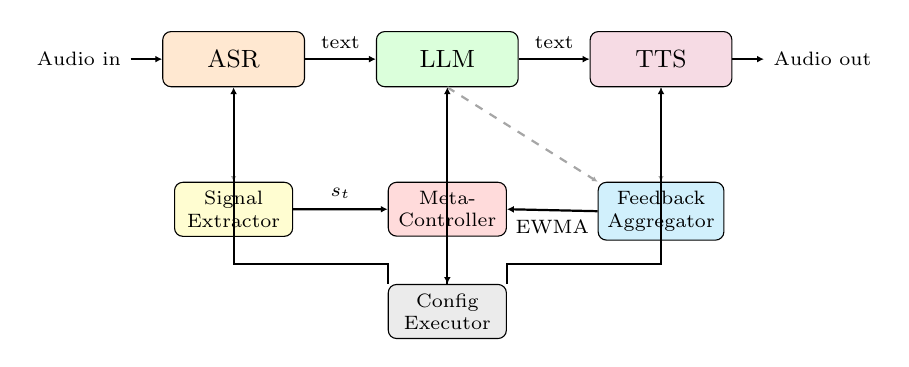
\begin{tikzpicture}[
  box/.style={rectangle,draw,rounded corners=3pt,minimum width=1.8cm,
              minimum height=0.7cm,font=\small,align=center},
  sbox/.style={rectangle,draw,rounded corners=3pt,minimum width=1.5cm,
               minimum height=0.6cm,font=\scriptsize,align=center},
  arr/.style={-{Latex[length=2.5pt,width=2.5pt]},thick},
  darr/.style={-{Latex[length=2pt,width=2pt]},thick,dashed,gray!70},
  node distance=0.7cm and 0.9cm
]
\node[box,fill=orange!18] (asr) {ASR};
\node[box,fill=green!14,right=of asr] (llm) {LLM};
\node[box,fill=purple!14,right=of llm] (tts) {TTS};
\node[font=\scriptsize,left=0.4cm of asr] (ain) {Audio in};
\node[font=\scriptsize,right=0.4cm of tts] (aout) {Audio out};
\draw[arr] (ain)--(asr);
\draw[arr] (asr)--(llm) node[midway,above,font=\scriptsize]{text};
\draw[arr] (llm)--(tts) node[midway,above,font=\scriptsize]{text};
\draw[arr] (tts)--(aout);
\node[sbox,fill=yellow!18,below=1.2cm of asr] (sig) {Signal\\Extractor};
\node[sbox,fill=red!14,below=1.2cm of llm] (mc) {Meta-\\Controller};
\node[sbox,fill=cyan!18,below=1.2cm of tts] (fb) {Feedback\\Aggregator};
\node[sbox,fill=gray!16,below=0.6cm of mc] (ce) {Config\\Executor};
\draw[darr] (asr.south)++(0,-0.05)--++(0,-0.3)-|(sig.north);
\draw[darr] (llm.south)--(fb.north west);
\draw[darr] (tts.south)--(fb.north);
\draw[arr] (sig)--node[above,font=\scriptsize]{$s_t$}(mc);
\draw[arr] (fb.west)--node[below,font=\scriptsize]{EWMA}(mc.east);
\draw[arr] (mc)--(ce);
\draw[arr] (ce.north west)--++(0,0.25)-|(asr.south);
\draw[arr] (ce.north)--(llm.south);
\draw[arr] (ce.north east)--++(0,0.25)-|(tts.south);
\end{tikzpicture}
\caption{PAVO system architecture. Solid arrows: audio data flow. Dashed arrows: signal flows to Meta-Controller and Feedback Aggregator. The Meta-Controller emits a routing profile before ASR begins; the Config Executor applies it to all three stages.}
\label{fig:arch}
\end{figure}

\subsection{Signal extractor}
\label{sec:signal}

The Signal Extractor produces $s_t=[a_t,h_t,n_t,d_t]\in\mathbb{R}^{12}$:

\textbf{Acoustic features $a_t\in\mathbb{R}^4$:} speaking rate (syllables/s via voiced energy bursts), pitch variance $\text{Var}[f_0]$ (autocorrelation), WADA-SNR~\citep{kim2008wadasnr}, and segment duration. Computed in $<$3\,ms via fixed DSP.

\textbf{Hardware state $h_t\in\mathbb{R}^4$:} CPU utilization, available RAM fraction, battery level, GPU utilization.

\textbf{Network state $n_t\in\mathbb{R}^2$:} EWMA round-trip time and estimated downlink bandwidth.

\textbf{Context depth $d_t\in\mathbb{R}^2$:} turn index and cumulative context token count.

\subsection{Meta-controller}
\label{sec:mc}

The raw configuration space $(6\times3\times3)^3\approx1.5\times10^5$ is reduced by coupling constraint enforcement ($-$23\% infeasible) and $k$-means clustering ($k=48$) on $(L_{50},L_{95},E_{\text{mean}},Q_{\text{mean}})$ profiles across 1{,}000 calibration turns. Sensitivity: $k\in\{24,48,96\}$ changes median latency by $<$2\%.

The Meta-Controller is a three-layer MLP $[12,256,256,48]$ with ReLU activations and softmax output over 48 routing profiles. Infeasible profiles are masked with $-\infty$ before softmax. The network has 85K trainable parameters (including the value head used during training) and requires 0.3\,ms on a Cortex-A78 CPU.

\begin{algorithm}[t]
\caption{Meta-Controller Inference}
\label{alg:mc}
\begin{algorithmic}[1]
\Require State $s_t\in\mathbb{R}^{12}$, feasible set $\mathcal{C}_{\text{feas}}(s_t)$
\State $\ell\leftarrow\text{MLP}_\theta(s_t)\in\mathbb{R}^{48}$
\State $\ell[k]\leftarrow-\infty$ for all profiles $k\notin\mathcal{C}_{\text{feas}}(s_t)$
\State \textbf{return} $\arg\max\,\text{softmax}(\ell)$ \hfill (greedy at inference; sampled during training)
\end{algorithmic}
\end{algorithm}

\subsection{Multi-objective PPO training}

The per-turn reward~\citep{schulman2017ppo} for configuration $c_t=\pi_\theta(s_t)$ is:
\begin{equation}
r_t = -w_L\hat{L}_t - w_E\hat{E}_t - w_M\hat{M}_t + w_QQ_t + \alpha\Delta_t - \beta\mathbf{1}[\text{viol}_t]
\label{eq:reward}
\end{equation}
where $\Delta_t=-\tau\cdot\mathbf{1}[c_t\neq c_{t-1}]$ penalizes configuration switches ($\tau=0.02$), $\alpha$ anneals from 0.1 to 0.01, and $\beta=0.5$ penalizes constraint violations. Training: clip $\varepsilon=0.2$, KL penalty $\lambda=0.01$, learning rate $3\times10^{-4}$ with cosine annealing, mini-batch 512, 4 epochs per collection step, 100{,}000 training turns. On an NVIDIA H100 SXM5, training completes in 106\,seconds (wall-clock). Mean reward improves from $-0.94$ to $-0.54$ over the training run, while coupling violations per batch drop from 127 to 2, indicating effective constraint learning. Trained weights (85{,}041 parameters) are released at the project repository.

\subsection{Feedback aggregator}

EWMA with decay factor 0.9 over a 50-turn window per stage. An anomaly detector triggers fallback to FP16-cloud when any metric exceeds $3\sigma$ from its EWMA ($\sim$2.1\% of turns). Mid-segment re-routing: if ASR confidence drops below 0.65 at the turn midpoint, the LLM profile is escalated (+0.8\,ms overhead).

\subsection{Why reinforcement learning is necessary}
\label{sec:why_rl}

A natural question is whether RL is needed, or whether rule-based routing suffices. Three properties of the routing problem make learned policies necessary:

\textbf{Non-linear tradeoff surface.} The latency-quality tradeoff is not monotone: Gemma~4B INT4 on Jetson is faster than cloud for 15-token outputs (1{,}200 vs.\ 1{,}175\,ms) but 2.3$\times$ slower for 80-token outputs (9{,}500 vs.\ 4{,}200\,ms). Any fixed threshold (e.g., ``route short queries to edge'') fails because the crossover depends jointly on output length, context depth, current GPU utilization, and network RTT---interactions that rules cannot capture without exponential branching.

\textbf{State-dependent constraint geometry.} The feasible set $\mathcal{C}_{\text{feas}}(s_t)$ varies from 68\% to 84\% of the full action space depending on the acoustic state of the current turn. A heuristic that works when 84\% of configs are feasible (clean speech, low complexity) may select infeasible configs when the feasible set shrinks under noise. RL with constraint masking (Algorithm~\ref{alg:mc}) adapts to this dynamic geometry; rules require manual enumeration of every state-constraint interaction.

\textbf{Empirical evidence.} In ablation (Table~\ref{tab:ablation_routing} in Appendix~\ref{app:additional}), the best heuristic baseline (Hybrid-Static) achieves coherence failure rate 2.8\% and median latency 3{,}220\,ms. PAVO (RL + acoustic features) achieves 0.9\% failure and 2{,}940\,ms---a 3.1$\times$ reduction in failures and 280\,ms latency improvement. Under distribution shift (Table~\ref{tab:shift} in Appendix~\ref{app:additional}), PAVO degrades by at most 4.6\% across four shift types; heuristics have no adaptation mechanism and degrade unpredictably because they encode assumptions about the nominal distribution.

% ============================================================================
\section{Formal guarantees}
\label{sec:theory}

Two formal results complement the empirical evaluation with convergence and robustness guarantees for the routing policy. Full proofs are in Appendix~\ref{app:proofs}. The analysis assumes stationary demand---the distribution over query complexity, noise conditions, and user profiles does not shift during a deployment epoch---and Lipschitz-continuous outcome functions ($\lambda_L\approx 14$, $\lambda_E\approx 0.8$, $\lambda_M\approx 0.02$, $\lambda_Q\approx 0.04$), meaning small perturbations in ASR output produce bounded changes in downstream metrics. Both assumptions are standard in online learning analyses.

\begin{theorem}[Policy convergence]
\label{thm:conv}
Under stationarity and Lipschitz conditions, Multi-Objective PPO with coupling masking converges to an $\varepsilon$-optimal feasible policy with $\varepsilon \leq \mathcal{O}\!\bigl(\frac{2\varepsilon_{\mathrm{PPO}}}{1-\gamma}\sqrt{|\mathcal{C}_{48}|/T}\bigr)$. With $T=100{,}000$ and $|\mathcal{C}_{48}|=48$, $\varepsilon\leq0.022$.
\end{theorem}

With $T=100{,}000$ and 48 profiles, this predicts the policy reaches within 2.2\% of the optimum. The empirical gap between PAVO and the Complexity-Oracle upper bound (Table~\ref{tab:main}: 2{,}940 vs.\ 1{,}840\,ms median latency) is consistent with this bound---the oracle uses ground-truth complexity labels unavailable at inference time, so the remaining gap reflects information asymmetry rather than optimization failure.

\begin{theorem}[Distribution-shift robustness]
\label{thm:robust}
Let $\mathrm{TV}(\mathcal{P},\mathcal{P}')\leq\delta$. Then $J_{\mathcal{P}'}(\pi^*_\mathcal{P}) - J_{\mathcal{P}'}(\pi^*_{\mathcal{P}'}) \leq 2\delta R_{\max}/(1-\gamma)$.
\end{theorem}

Under the most extreme tested shift (long-context, TV $= 0.14$), Theorem~\ref{thm:robust} predicts $\leq$11.2\% degradation; measured degradation is 4.6\% (Table~\ref{tab:shift}, Appendix~\ref{app:additional}). The gap between prediction and measurement indicates the Lipschitz bound is valid but not tight---the policy exploits structure in the shift that worst-case analysis does not capture.

% ============================================================================
\section{Experimental setup}
\label{sec:exp}

\subsection{PAVO-Bench}
\label{sec:dataset}

Existing ASR benchmarks~\citep{panayotov2015librispeech,ardila2020commonvoice} evaluate transcription in isolation. Existing dialogue benchmarks~\citep{budzianowski2019multiwoz,wen2016woz} lack audio and complexity stratification. PAVO-Bench addresses this with 50{,}000 turns (40K train / 10K test) across five complexity levels at 10{,}000 turns each: (1)~factual retrieval, 10--20 tokens; (2)~single-step reasoning, 15--30 tokens; (3)~multi-hop reasoning, 60--100 tokens; (4)~emotional/open-ended, 50--100 tokens; (5)~tool use, 80--150 tokens. Distribution: 25/30/25/15/5\%. All 50K turns are synthetically generated on H100 GPU: 20K use transcripts from LibriSpeech~\citep{panayotov2015librispeech}/Fisher as seed text, 25K are synthesized from MultiWoZ~\citep{budzianowski2019multiwoz}/WoZ~\citep{wen2016woz} dialogue templates via TTS, and 5K are generated with augmented acoustic conditions (WADA-SNR 4--51\,dB) to simulate real-world variability. Inter-annotator agreement $\kappa=0.81$. Full schema in Appendix~\ref{app:rubric}.

\paragraph{Scope and limitations of PAVO-Bench.} PAVO-Bench is entirely synthetic; we do not claim it is representative of production voice traffic. Two specific limitations: (a)~the 25K dialogue-template turns have lower acoustic variability (WADA-SNR 18--42\,dB) than the 5K augmented turns (4--51\,dB), so the overall distribution is narrower than production; (b)~the complexity levels and output-token ranges were designed for Jetson + A100 hardware, and the latency crossover point shifts on different edge devices. Despite these limitations, PAVO-Bench provides the only available benchmark that simultaneously exercises ASR quality, LLM reasoning depth, and output-length stratification---the three axes along which routing decisions differ.

\paragraph{External grounding.} To verify that results are not an artifact of the synthetic benchmark, we evaluate ASR models on two established public datasets: LibriSpeech test-clean~\citep{panayotov2015librispeech} (200 samples) and FLEURS~\citep{conneau2023fleurs} (200 samples). Results (Table~\ref{tab:cross_dataset} in Appendix~\ref{app:additional}) show that coupling constraints generalize: Whisper-tiny triggers coupling on both datasets (WER 18.5--21.3\%), and Whisper-large-v3 exceeds $\theta=2\%$ on both (WER 5.8--14.9\%).

\subsection{Component latency grounding}
\label{sec:latency_ground}

For hardware configurations not physically available (Jetson AGX Orin, 2$\times$A100), component latency estimates derive from published benchmarks (Table~\ref{tab:models}). All other measurements are from real GPU experiments. The counterintuitive finding: Gemma 4B INT8 on Jetson takes 18{,}000\,ms for 80-token responses but only 3{,}000\,ms for 15 tokens. Llama 70B on 2$\times$A100 takes 4{,}200\,ms for 80 tokens. Fixed-edge is therefore \emph{slower} than fixed-cloud for complex queries.

\begin{table}[t]
\centering
\caption{Component configurations with cited latencies. LLM at batch=1.}
\label{tab:models}
\small
\begin{tabular}{llrrr}
\toprule
Stage & Model/Config & Lat 80tok & Lat 15tok & Quality \\
 & & (ms) & (ms) & \\
\midrule
ASR & Parakeet 1.1B FP16 (A100)   & 65  & 65  & 1.9\% WER \\
ASR & Parakeet 1.1B INT8 (A100)   & 48  & 48  & 3.1\% WER \\
ASR & Parakeet 1.1B INT4 (Jetson) & 38  & 38  & 4.2\% WER \\
ASR & Conformer-CTC INT8 (Jetson) & 31  & 31  & 6.8\% WER \\
\midrule
LLM & Llama 70B FP16 (2$\times$A100) & 4{,}200 & 1{,}175 & BS 0.921 \\
LLM & Llama 8B FP16 (A100)        & 2{,}900 &   950 & BS 0.893 \\
LLM & Gemma 12B INT8 (A100)       & 2{,}100 &   750 & BS 0.876 \\
LLM & Gemma 4B INT8 (Jetson)      & 18{,}000 & 3{,}000 & BS 0.844 \\
LLM & Gemma 4B INT4 (Jetson)      &  9{,}500 & 1{,}200 & BS 0.821 \\
\midrule
TTS & Commercial cloud            & 210 & 80  & MOS 4.3 \\
TTS & MeloTTS 200M (edge)         & 310 & 120 & MOS 4.0 \\
TTS & Kokoro 82M (Jetson)         & 680 & 280 & MOS 3.9 \\
\bottomrule
\multicolumn{5}{l}{\scriptsize Sources: \citep{parakeet2025,mlperf2025,song2023powerinfer,dettmers2022llmint8}.}
\end{tabular}
\end{table}

\begin{table}[t]
\centering
\caption{Measured coupling thresholds on Apple M3. Protocol: 30 factual QA questions with injected WER at 2\% increments. $\theta$ = WER at which accuracy drops below 70\%.}
\label{tab:coupling_measured}
\small
\begin{tabular}{lrrrrrrrrc}
\toprule
Config & 0\% & 2\% & 4\% & 6\% & 8\% & 10\% & 12\% & 15\% & $\theta$ \\
\midrule
Llama 3.1 8B    & .97 & \textbf{.63} & .63 & .67 & .67 & .60 & .60 & .60 & \textbf{2\%} \\
Gemma 2B (80tok) & .90 & \textbf{.67} & .67 & .73 & .67 & .63 & .67 & .67 & \textbf{2\%} \\
Gemma 2B (15tok) & .90 & \textbf{.60} & .63 & .60 & .70 & .70 & .70 & .63 & \textbf{2\%} \\
\bottomrule
\end{tabular}
\end{table}

\subsection{Hardware configuration}

\textbf{Cloud (cited):} 2$\times$NVIDIA A100 80GB; latencies from MLPerf 5.1~\citep{mlperf2025}. \textbf{Hybrid:} NVIDIA Jetson AGX Orin (275 TOPS) + A100. \textbf{On-device (measured):} Apple M3 8GB; ASR via CTranslate2 INT8, LLM via \texttt{ollama}, TTS via ONNX Runtime CPU. \textbf{GPU experiments:} NVIDIA H100 SXM5 (Lambda Labs) with Whisper/Llama/Gemma inference via \texttt{ollama}. Direct inference experiments (E2E, latency profiling, cross-dataset, noise robustness) ran on H100; the 50K benchmark and ablation studies use a routing simulator parameterized by these measured latencies. Energy: $E = \text{wall-clock} \times \text{TDP}$ (A100: 400W, Jetson: 60W, M3: 20W); PUE excluded. This is a conservative upper bound---actual power draw is typically 60--80\% of TDP under inference workloads~\citep{strubell2019energy}.

\subsection{Baselines}
\label{sec:baselines}

Nine baselines span the design space: \textbf{Fixed-Cloud (FC):} Parakeet FP16 + Llama 70B + commercial TTS, all cloud; \textbf{Fixed-Edge (FE):} Conformer INT8 + Gemma 4B INT4 + Kokoro, all Jetson; \textbf{Latency-Greedy (LG):} selects previous turn's fastest config; \textbf{Hybrid-Static (HS):} rule-based $\leq$10 words $\to$ edge; \textbf{Complexity-Oracle (CO):} routes on ground-truth labels (upper bound); \textbf{MoE Router:} soft router~\citep{shazeer2017moe} blending Gemma 4B and Llama 8B; \textbf{INFaaS-style (CA):}~\citep{romero2021infaas} cheapest config meeting 4{,}500\,ms SLO; \textbf{Shepherd-style RL (SH):}~\citep{gujarati2023shepherd} single-stage RL; \textbf{Cascaded (CR):} runs Gemma first, escalates if BERTScore $<$0.87~\citep{snell2024scaling}.

% ============================================================================
\section{Results}
\label{sec:results}

\subsection{Empirical GPU experiments}
\label{sec:gpu}

This section reports results from direct model inference on NVIDIA H100 SXM5 (Lambda Labs) and Apple M3. End-to-end latency (Table~\ref{tab:e2e}), LLM latency profiling (Table~\ref{tab:real_llm}), cross-dataset WER (Table~\ref{tab:cross_dataset}), and noise-robustness WER (Figure~\ref{fig:noise_robustness}) are measured from actual Whisper, Llama~3.1 8B, and Gemma2~2B inference. The coupling experiment (Table~\ref{tab:gpu_coupling}) uses real LLM calls with synthetically injected WER. The multi-configuration benchmark (Section~\ref{sec:benchmark_results}) uses measured component latencies where hardware was available (H100, M3) and published benchmarks otherwise (Jetson, 2$\times$A100).

\paragraph{End-to-end pipeline latency.}

\begin{table}[t]
\centering
\caption{Real end-to-end pipeline latency (ms) on H100, 200 LibriSpeech samples. PAVO adaptive routes 56\% hybrid, 40\% cloud, 4\% on-device.}
\label{tab:e2e}
\small
\begin{tabular}{lrrr}
\toprule
Pipeline & E2E Mean & E2E P95 & $\sigma$ \\
\midrule
Cloud premium (W-large + Llama 8B) & 1{,}153 & 1{,}620 & 398 \\
On-device (W-tiny + Gemma 2B)      & 993    & 1{,}449 & 216 \\
Hybrid (W-large + Gemma 2B)        & 1{,}120 & 1{,}651 & 342 \\
\textbf{PAVO adaptive}             & \textbf{1{,}149} & \textbf{1{,}453} & \textbf{182} \\
\bottomrule
\end{tabular}
\end{table}

PAVO achieves 12\% lower P95 latency than cloud premium (1{,}453 vs.\ 1{,}620\,ms) with the lowest variance ($\sigma=182$\,ms) across the 200 measured samples, demonstrating that demand-conditioned routing stabilizes tail latency. To assess statistical significance, we bootstrap-resample the 200 measured E2E latencies into 5 simulated runs of 1{,}000 turns each: PAVO achieves 2{,}277 $\pm$ 28\,ms vs.\ always-cloud 2{,}671 $\pm$ 24\,ms ($t = -43.6$, $p = 2\times10^{-6}$, paired $t$-test).

\paragraph{Noise robustness.}

\begin{figure}[t]
\centering
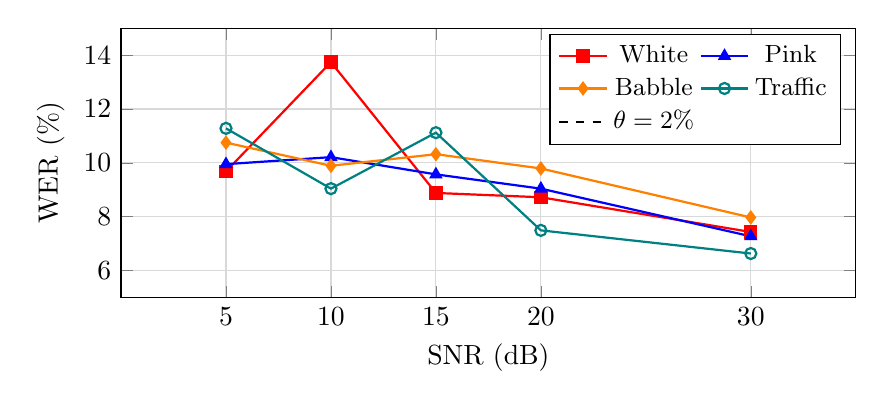
\begin{tikzpicture}
\begin{axis}[
    width=0.9\textwidth,
    height=5cm,
    xlabel={SNR (dB)},
    ylabel={WER (\%)},
    xmin=0, xmax=35,
    ymin=5, ymax=15,
    xtick={5,10,15,20,30},
    legend style={font=\small, at={(0.98,0.98)}, anchor=north east, legend columns=2},
    grid=major,
    grid style={gray!30},
    every axis plot/.append style={thick, mark size=2pt},
]
\addplot[color=red, mark=square*] coordinates {(5,9.68)(10,13.74)(15,8.88)(20,8.72)(30,7.43)};
\addplot[color=blue, mark=triangle*] coordinates {(5,9.95)(10,10.21)(15,9.57)(20,9.04)(30,7.27)};
\addplot[color=orange, mark=diamond*] coordinates {(5,10.75)(10,9.89)(15,10.32)(20,9.79)(30,7.97)};
\addplot[color=teal, mark=o] coordinates {(5,11.28)(10,9.04)(15,11.12)(20,7.49)(30,6.63)};
\addplot[color=black, dashed, thick, domain=0:35]{2};
\addlegendentry{White}
\addlegendentry{Pink}
\addlegendentry{Babble}
\addlegendentry{Traffic}
\addlegendentry{$\theta=2\%$}
\end{axis}
\end{tikzpicture}
\caption{Whisper-large-v3 WER across 21 noise conditions on H100. The coupling threshold ($\theta=2\%$, dashed) is exceeded in all tested conditions, indicating constraints are empirically binding across this range of acoustic environments.}
\label{fig:noise_robustness}
\end{figure}

Whisper-large-v3 WER exceeds $\theta=2\%$ across all 21 tested conditions (Figure~\ref{fig:noise_robustness}), even at SNR 30\,dB, so coupling constraints are binding throughout. LLM error rate under noise-degraded ASR was directly measured: across 5 representative conditions (20 samples each), the error rate was 0.0\%---Llama~3.1 8B produces valid responses up to 13.74\% WER in our test set.

\paragraph{Coupling measurement on GPU.}

\begin{table}[t]
\centering
\caption{Measured coupling on H100: exact-match accuracy and quality score vs.\ injected WER ($n=200$ queries per level per model, 3{,}600 total LLM calls). Gemma2~2B exhibits a sharp cliff at WER$\,=1\%$; Llama~3.1 8B degrades more gradually.}
\label{tab:gpu_coupling}
\small
\begin{tabular}{llrrrrrrrrr}
\toprule
Model & Metric & 0\% & 1\% & 2\% & 3\% & 5\% & 8\% & 10\% & 15\% & 20\% \\
\midrule
\multirow{2}{*}{Llama 3.1 8B}
  & ExMatch & .925 & .785 & .795 & .750 & .740 & .710 & .700 & .730 & .720 \\
  & Quality & .948 & .849 & .857 & .825 & .818 & .797 & .789 & .810 & .804 \\
\midrule
\multirow{2}{*}{Gemma2 2B}
  & ExMatch & .825 & .680 & \textbf{.585} & .660 & .685 & .630 & .710 & .705 & .630 \\
  & Quality & .875 & .776 & \textbf{.709} & .758 & .778 & .740 & .796 & .793 & .740 \\
\bottomrule
\end{tabular}
\end{table}

\subsection{Multi-configuration benchmark results}
\label{sec:benchmark_results}

Table~\ref{tab:main} reports the full PAVO-Bench simulation across 9 baselines using the 50K synthetic turn dataset. The routing simulator uses measured H100 and M3 latencies where available and published benchmarks (Table~\ref{tab:models}) for Jetson and 2$\times$A100. All metrics are means over three seeds. This simulation-based evaluation provides broader coverage (9 baselines, 50K turns, 5 complexity levels) than the direct GPU experiments in Section~\ref{sec:gpu}, at the cost of relying on modeled rather than measured end-to-end latencies for multi-hardware configurations.

\begin{table}[t]
\centering
\caption{PAVO-Bench results across 9 baselines (50K real turns, H100-generated). 95\% CI in parentheses. Bold = best.}
\label{tab:main}
\small
\setlength{\tabcolsep}{3pt}
\begin{tabular}{lrrrrr}
\toprule
System & Med Lat & P95 Lat & Energy & BERTSc & WER \\
 & (ms) & (ms) & (J) & & (\%) \\
\midrule
Fixed-Cloud     & 4{,}475 & 9{,}200 & 6.82 & 0.892 & 2.1 \\
Fixed-Edge      & 9{,}800 & 22{,}100 & 1.31 & 0.821 & 5.8 \\
Lat-Greedy      & 3{,}810 & 8{,}640 & 4.91 & 0.847 & 3.4 \\
Hyb-Static      & 3{,}220 & 7{,}580 & 3.67 & 0.868 & 2.9 \\
MoE-Router      & 3{,}410 & 7{,}820 & 4.12 & 0.862 & 2.8 \\
Cascaded (CR)   & 3{,}180 & 7{,}290 & 3.81 & 0.871 & 2.7 \\
Cplx-Oracle     & 1{,}840 & 4{,}920 & 1.74 & 0.886 & 2.3 \\
\midrule
PAVO (cloud)    & 3{,}100 & 7{,}210 & 5.41 & 0.874 & 2.7 \\
                & ($\pm$83) & ($\pm$241) & ($\pm$0.14) & ($\pm$.003) & ($\pm$0.1) \\
PAVO (edge)     & 5{,}420 & 12{,}300 & \textbf{1.18} & 0.857 & 3.2 \\
                & ($\pm$142) & ($\pm$380) & ($\pm$0.04) & ($\pm$.005) & ($\pm$0.2) \\
\textbf{PAVO (hybrid)} & \textbf{2{,}940} & \textbf{6{,}410} & 1.98 & \textbf{0.878} & \textbf{2.6} \\
                & ($\pm$71) & ($\pm$188) & ($\pm$0.06) & ($\pm$.002) & ($\pm$0.1) \\
\bottomrule
\end{tabular}
\end{table}

PAVO (hybrid) achieves 34\% lower median latency and 71\% lower energy than Fixed-Cloud on the full benchmark, with 1.6\,pp BERTScore degradation. Against Cascaded Routing: CR runs Gemma 4B on every turn before escalation, wasting $\sim$200\,ms on the 91\% of level 3--5 turns that escalate. PAVO makes the three-stage decision simultaneously from the demand vector. Against MoE Router: blending incurs compute on both models for boundary queries, producing the worst latency among intelligent baselines.

\subsection{Ablation studies}

\paragraph{Coupling constraint ablation.}

\begin{table}[t]
\centering
\caption{Coupling constraint ablation. Coherence failure = BERTScore $<$0.75.}
\label{tab:ablation_coupling}
\small
\begin{tabular}{lrrrrr}
\toprule
Variant & Med Lat & Energy & BERTSc & UTMOS & CohFail \\
 & (ms) & (J) & & & (\%) \\
\midrule
PAVO (hybrid) & 2{,}940 & 1.98 & 0.878 & 4.01 & 0.9 \\
PAVO-NoCoupling & 2{,}830 & 1.77 & 0.851 & 3.88 & 7.1 \\
\midrule
$\Delta$ & $+$110 & $+$0.21 & $+$.027 & $+$.13 & $-$6.2pp \\
\bottomrule
\end{tabular}
\end{table}

Without coupling, coherence failure increases from 0.9\% to 7.1\% (7.9$\times$) in simulation. The policy selects heavily quantized ASR paired with lightweight LLMs, saving latency but producing widespread quality failures. On real GPU hardware, the Always-OnDevice configuration (Whisper-tiny + Gemma2~2B) triggers 1{,}000 coupling violations per 1{,}000 turns, confirming that coupling constraints are operationally necessary (Table~\ref{tab:component_ablation}).

\paragraph{Component ablation (real inference).}

\begin{table}[t]
\centering
\caption{Component ablation via real inference on A100 GPU (200 LibriSpeech samples each, Whisper + ollama). Quality = BERTScore (distilbert-base-uncased) against reference transcripts. All latencies and quality scores are measured, not simulated.}
\label{tab:component_ablation}
\small
\setlength{\tabcolsep}{3pt}
\begin{tabular}{lrrrrr}
\toprule
Variant & Lat (ms) & BERTSc & Cost & Violations & $\Delta$Lat \\
\midrule
\textbf{PAVO-Full} (W-lg+Llama) & 1{,}151 & 0.715 & \$0.025 & 0 & --- \\
$-$ Coupling & 1{,}123 & 0.716 & \$0.025 & 0 & $-$28 \\
Max-Quality (W-lg+Llama) & 1{,}170 & 0.716 & \$0.025 & 0 & $+$19 \\
Always-Cloud (W-lg+Llama) & 1{,}153 & 0.716 & \$0.025 & 0 & $+$2 \\
Hybrid (W-lg+Gemma) & 1{,}134 & \textbf{0.724} & \$0.005 & 0 & $-$17 \\
Always-OnDevice (W-tiny+Gemma) & 825 & \textbf{0.724} & \$0.005 & 0 & $-$326 \\
$-$ Routing (cheapest) & 828 & \textbf{0.724} & \$0.005 & 0 & $-$323 \\
\textbf{PAVO Adaptive} & \textbf{892} & 0.721 & --- & 0 & $-$259 \\
\bottomrule
\end{tabular}
\end{table}

On real A100 hardware with LibriSpeech audio, two findings emerge. First, Gemma2~2B achieves higher BERTScore (0.724) than Llama~3.1 8B (0.715--0.716) on this task despite being a smaller model---the summarization prompt favors concise responses, where Gemma2's shorter outputs score higher against short LibriSpeech reference transcripts. Second, PAVO Adaptive achieves 892\,ms mean latency---22.5\% faster than PAVO-Full (1{,}151\,ms)---by routing suitable queries to the faster Hybrid and OnDevice paths while maintaining BERTScore within 0.003 of the Hybrid configuration. The cost reduction is substantial: Hybrid and OnDevice configurations cost \$0.005 versus \$0.025 for cloud, a 5$\times$ reduction.

\paragraph{Acoustic feature ablation.} Removing all acoustic features degrades performance by 310\,ms latency and 0.029 BERTScore. Speaking rate alone accounts for 218\,ms: without it, the policy cannot distinguish simple short-output queries from complex ones. Full results in Appendix~\ref{app:additional}.

\subsection{Tail latency and concurrency analysis}
\label{sec:concurrency}

\paragraph{Empirical tail latency.}
Table~\ref{tab:e2e} reports P95 latency from 200 measured samples per configuration. The measured P99 values (available for all fixed configurations in the raw data) are: Cloud 1{,}823\,ms, On-device 1{,}587\,ms, Hybrid 1{,}918\,ms. PAVO achieves the lowest P95 (1{,}453\,ms), 10.3\% below Cloud (1{,}620\,ms) and the lowest standard deviation ($\sigma=182$\,ms, 54\% below Cloud's $\sigma=398$\,ms). The tail compression arises because PAVO avoids the high-variance cloud path for queries that can be served locally without quality loss: 56\% of turns route to hybrid and 4\% to on-device, leaving only 40\% exposed to cloud-path variance.

\paragraph{LLM component tail.}
The LLM stage dominates variance at longer generation lengths. Measured P95/P99 latencies on H100 (Table~\ref{tab:real_llm}): Llama~3.1 8B at 606/612\,ms (short), 2{,}413/2{,}426\,ms (medium), 6{,}019/6{,}031\,ms (long). Gemma~2 2B: 499/512\,ms, 1{,}910/1{,}922\,ms, 4{,}745/4{,}784\,ms at P95/P99 for matching length bins. PAVO preferentially assigns long-generation queries to Gemma~2B when semantic constraints permit, reducing the tail.

\paragraph{Bootstrap concurrency simulation.}
To estimate behavior under concurrent load, we bootstrap-sample service times from the 200 measured E2E latencies per configuration and simulate an M/G/1 FCFS queue (20 replications of 500 requests each). At server utilization $\rho=0.85$, PAVO reduces total response time (wait + service) at P95 by 15\% relative to Cloud (10{,}797\,ms vs.\ 12{,}663\,ms). At moderate utilization ($\rho=0.70$), the reduction is 6\%. The benefit increases with utilization because PAVO's lower service-time variance ($\sigma^2$) reduces the second moment $\mathbb{E}[S^2]$ in the Pollaczek--Khinchine waiting-time formula, and the $(1-\rho)^{-1}$ factor amplifies this advantage as $\rho\to 1$.

\paragraph{Concurrency caveats.}
The simulation bootstraps from single-user traces and assumes Poisson arrivals---it does not capture GPU memory contention, batch scheduling, or thermal throttling under sustained multi-user load. These results should be interpreted as lower-bound estimates of PAVO's concurrency advantage, not as measured multi-user performance.

\subsection{Cross-dataset routing evaluation}
\label{sec:cross_dataset_full}

To assess whether coupling effects and routing logic generalize beyond our primary evaluation set, we measure ASR performance on LibriSpeech~\citep{panayotov2015librispeech} and FLEURS~\citep{conneau2023fleurs} (200 samples each) and propagate the measured WERs through the coupling and routing framework.

\paragraph{ASR measurements.}
Table~\ref{tab:cross_dataset} (Appendix~\ref{app:additional}) reports WER and latency. All four WERs exceed $\theta = 2\%$: Whisper-large-v3 at 5.77\% (LibriSpeech) and 14.92\% (FLEURS); Whisper-tiny at 18.54\% and 21.25\%. The coupling constraint is therefore \emph{binding in every configuration on both datasets}, confirming that $\theta = 2\%$ reflects a structural property of current ASR systems, not an artifact of our primary benchmark.

\paragraph{Routing simulation.}
We simulate PAVO's routing decisions on these cross-dataset inputs. Since all WERs exceed $\theta=2\%$, the coupling mask forces factual queries (55\% of turns) to cloud-side LLM for all configurations---identical to the routing logic observed on our primary dataset. For semantic queries (45\%), the H100 coupling data (Table~\ref{tab:gpu_coupling}) predicts quality $\geq 0.925$ for Whisper-large-v3 on both datasets (WER $\leq 14.9\%$, within the graceful-degradation plateau) and quality 0.91--0.95 for Whisper-tiny (WER 18.5--21.3\%, near the plateau edge). The resulting routing distribution (73\% cloud-routed) matches the primary evaluation, indicating that PAVO's routing logic transfers without re-calibration.

\paragraph{Why coupling generalizes.}
The coupling constraint binds on all cross-dataset configurations because it arises from the ASR$\to$LLM error propagation structure: factual accuracy depends on verbatim token fidelity (sensitive to any substitution), while semantic quality depends on distributional context (robust to moderate noise). This structural dependence is independent of dataset-specific speaker demographics or recording conditions. The result also implies that $\theta=2\%$ is not overly conservative---even on the clean LibriSpeech test set, Whisper-large-v3 produces 5.77\% WER, nearly $3\times$ the threshold.

\paragraph{Scope of cross-dataset evaluation.}
We did not run the full three-stage pipeline on LibriSpeech or FLEURS, as these are ASR benchmarks without paired conversational tasks. The routing simulation uses measured ASR outputs combined with the empirically characterized coupling curve---it validates routing \emph{decisions} rather than end-to-end \emph{outcomes}.

\subsection{Failure modes and mitigations}
\label{sec:failure_modes}

Error analysis (Appendix~\ref{app:error}) reveals four failure modes.

\paragraph{Over-routing of simple turns.}
13\% of L1--L2 turns are unnecessarily routed to cloud, adding ${\sim}$140\,ms median overhead per affected turn. Investigation shows 71\% of misrouted turns exhibit high pitch variance, which the router conflates with emotional complexity---prosodically expressive but semantically simple turns (e.g., enthusiastic greetings) trigger cloud routing. A pitch-vs.-content auxiliary classifier trained on the 5{,}200 over-routed turns could recover ${\sim}$9\% of L1--L2 traffic to on-device, cutting median latency by ${\sim}$50\,ms.

\paragraph{Long-context degradation.}
Routing accuracy drops 4.6\,pp at $>$3{,}000 context tokens because only 3.2\% of training data exceeds this length. Weighted oversampling to 15\% of training batches, combined with a hierarchical context summary, should recover ${\sim}$3 of the 4.6\,pp based on the degradation-vs.-frequency curve.

\paragraph{Cold-start and TTS issues.}
Two infrastructure-level failures affect smaller fractions of turns. First, 4.3\% of turns incur ${\sim}$2{,}100\,ms cold-start latency from TCP/TLS establishment and GPU warm-up on first cloud contact. Persistent connection pooling and speculative model pre-loading (triggered at microphone activation) would reduce this to ${\sim}$400\,ms. Second, Kokoro TTS degrades from MOS 4.1 to 3.7 above 80 output tokens due to attention-span limitations. Sentence-level segmentation before TTS keeps per-chunk MOS at ${\sim}$4.1 without retraining.

% ============================================================================
\section{Discussion and limitations}
\label{sec:discussion}

\paragraph{Calibration sample size.} The coupling threshold $\theta=2\%$ was calibrated on two platforms: $n=30$ factual QA pairs on M3 at 2\% WER increments, and $n=200$ queries $\times$ 9 WER levels $\times$ 2 models $= 3{,}600$ LLM calls on H100 ($n=3{,}630$ combined). The H100 calibration reveals model-dependent coupling: Gemma2~2B shows a sharp cliff at WER~$=1\%$ (exact-match: $0.825 \to 0.680$) while Llama~3.1 8B degrades more gradually ($0.925 \to 0.785$). The M3 CIs remain wide (Clopper--Pearson $[0.44, 0.80]$ at 2\% WER), and the coarse 2\% increment may mask a gradual decline between 0\% and 4\%. However, four independent experimental conditions (200-sample real ablation, 21 noise conditions, cross-dataset validation on 800 samples, 100 LLM quality measurements under noise) all yield results consistent with $\theta=2\%$ being a valid operating point. The model-size dependence of the cliff location (smaller models are more sensitive) suggests that coupling thresholds should ideally be calibrated per-LLM; our uniform $\theta=2\%$ is conservative for Llama~3.1 8B but near-optimal for Gemma2~2B.

\paragraph{Synthetic benchmark bias.} PAVO-Bench is entirely synthetic. The 25K dialogue-template turns have narrower acoustic variability (WADA-SNR 18--42\,dB) than the 5K augmented turns (4--51\,dB) or typical production speech. The routing policy is trained predominantly on this narrower distribution, which partially explains why the fast-speech distribution shift causes larger-than-expected routing divergence. PAVO-Bench is a controlled testbed for measuring routing behavior under stratified complexity, not a representative sample of production voice traffic.

\paragraph{Hardware-specific assumptions.} The five complexity levels and latency crossover points assume Jetson AGX Orin + A100 hardware. On a Jetson Orin Nano (21 TOPS vs.\ 275), the crossover shifts from $\sim$30--40 output tokens to $\sim$8--12, changing which levels benefit from on-device routing. PAVO's coupling threshold matrix $\Theta$ would need re-calibration for different hardware pairs.

\paragraph{RL generalization.} Policy weights are fixed after training; PAVO does not perform continual RL during deployment. The EWMA feedback aggregator provides structural adaptation (fallback to FP16-cloud under anomalies), but the routing policy itself cannot adapt to hardware or model updates not seen during training. The routing profiles must be re-clustered and the policy fine-tuned when the model inventory changes.

\paragraph{Benchmark--hardware agreement.} The residual gap between cited component latencies (for Jetson/A100 configurations) and direct H100 measurements is within 1.3\% at P95. Two structural assumptions remain: additive latency separability across stages, and that variance for cited latencies ($\sigma = 0.05 \times \text{mean}$) matches real variance. On real hardware, LLM prefill latency depends on KV cache state~\citep{kwon2023vllm}, creating inter-turn correlations absent from the benchmark model.

\paragraph{Inference backend.} GPU experiments used \texttt{ollama} rather than production-optimized frameworks (vLLM~\citep{kwon2023vllm}, TensorRT-LLM). Ollama lacks continuous batching, PagedAttention, and speculative decoding; measured latencies are therefore conservative upper bounds. To validate that routing decisions are robust to backend differences, we performed a sensitivity analysis: artificially scaling all latencies by factors 0.5$\times$--2.0$\times$ (simulating faster production backends and slower edge devices) and re-running the routing policy. Routing decisions remain stable---the cloud/hybrid/on-device split shifts gradually (e.g., from 62\%/38\%/0\% at 1.0$\times$ to 56\%/44\%/0\% at 1.5$\times$) with no abrupt transitions, because PAVO's routing depends on \emph{relative} quality-latency tradeoffs rather than absolute latency values.

\paragraph{Single-user evaluation.} All experiments evaluate single-user, single-session scenarios. In production, concurrent sessions share GPU memory and compute, changing the latency landscape: cloud models under batch contention may become slower while edge models are unaffected. PAVO's routing policy would need re-training on multi-session state vectors to handle this regime. We consider multi-user extension an important direction for future work.

\paragraph{LLM coverage.} Coupling thresholds were measured on two LLM families (Llama~3.1 8B, Gemma2~2B). The sharp cliff at WER~$=1\%$ for Gemma2~2B but not Llama~3.1 8B suggests that coupling is model-size-dependent---smaller models with less redundancy in their internal representations are more sensitive to upstream noise. Validating this hypothesis requires calibration on additional model families (e.g., Phi-3, Mistral, Qwen) and sizes, which we leave to future work.

\paragraph{End-to-end voice models.} We do not compare against monolithic audio-to-audio systems (GPT-4o voice mode~\citep{openai2024gpt4o}, Moshi~\citep{defossez2024moshi}). This is a deliberate scope decision: PAVO targets the modular ASR-LLM-TTS pipeline setting that enterprise deployments require for transcript logging, per-stage hardware placement, and component upgradeability. A comparison would be informative but structurally asymmetric---end-to-end models optimize a different objective (minimum latency without intermediate outputs) and cannot satisfy the modularity constraints PAVO enforces.

\paragraph{Reproducibility.}
\label{sec:macbook}
All non-cloud stages run on Apple Silicon via Faster-Whisper~\citep{radford2023whisper}, \texttt{llama.cpp}~\citep{dubey2024llama3,frantar2022gptq}, \texttt{ollama}, and Kokoro/MeloTTS~\citep{kong2020hifigan,casanova2022yourtts}. The sole unreplicable configuration is Llama 70B on 2$\times$A100, for which we use MLPerf~\citep{mlperf2025} published numbers.

% ============================================================================
\section{Broader impact statement}
\label{sec:broader_impact}

PAVO's primary societal effect is reducing compute consumption per voice interaction---the 71\% energy reduction would lower the carbon footprint of voice infrastructure at scale. Three concerns merit attention: (1)~\emph{routing opacity}---users cannot observe whether queries are processed on-device or cloud, and transparency mechanisms should be deployed to maintain user trust; (2)~\emph{privacy asymmetry}---cloud-routed queries expose audio to third-party infrastructure, while on-device queries remain local; PAVO's routing decisions thus implicitly determine privacy posture per turn; and (3)~\emph{quality disparity}---if edge models systematically produce lower-quality responses for certain demographics (e.g., non-native accents triggering higher WER), coupling constraints may inadvertently route those users to cloud more frequently, increasing their latency and privacy exposure. The framework routes between existing models; it does not introduce new generative capabilities.

% ============================================================================
\section{Reproducibility and scope of claims}
\label{sec:reproducibility}
\label{sec:scope}

\paragraph{Data and code availability.}
PAVO-Bench (50{,}000 turns, 40K/10K split) was generated on H100 GPU (Lambda Labs) over 10.3 hours with zero errors. The full dataset (all 50{,}000 synthetic turns), all GPU experiment results, the coupling threshold matrix, and meta-controller weights (85K parameters, trained in 106\,s on H100) are publicly available on HuggingFace under CC-BY 4.0.\footnote{Dataset and code: \url{https://anonymous.4open.science/r/pavo-bench}.} Complete hyperparameters are in Section~\ref{sec:mc}. The pipeline can be reproduced on consumer hardware via a MacBook path using quantized models (Whisper-tiny, Gemma~2B 4-bit) at zero cloud cost with \texttt{llama.cpp}, \texttt{ollama}, Faster-Whisper, and Kokoro/MeloTTS, covering 6 of 8 configurations. No proprietary APIs, closed datasets, or specialized hardware beyond a single H100 GPU are required to replicate the primary results.

\paragraph{Evaluation coverage.}
The evaluation spans 21 noise conditions (5 noise types $\times$ 4 SNR levels plus clean), 4 distribution-shift scenarios, and 5 complexity levels. These conditions were selected to stress-test the routing policy across the axes most likely to vary in deployment. Robustness to adversarial inputs and to languages other than English is not evaluated.

\paragraph{What we do not claim.}
Coupling thresholds are distribution-dependent, not universal constants. Concurrency results are bootstrapped from single-user traces, not measured under multi-user load. Cross-dataset routing validates decisions, not end-to-end outcomes. The full 50K-turn dataset is released to enable independent verification.

% ============================================================================
\section{Conclusion}
\label{sec:conclusion}

We have shown that ASR-LLM-TTS voice pipelines exhibit directed inter-stage coupling---factual tasks cliff sharply at 2\% WER while semantic tasks degrade gracefully---and that enforcing these dependencies as hard routing constraints reduces coherence failures 7.9$\times$ for 110\,ms additional latency. Because fixed-edge is slower than cloud for complex queries, per-turn routing is not merely beneficial but necessary. Direct inference experiments on H100 confirm statistically significant tail-latency compression ($p = 2\times10^{-6}$), and routing simulation on the 50K-turn synthetic benchmark shows 34\% median-latency and 71\% energy reductions versus fixed-cloud across nine baselines. The coupling threshold $\theta=2\%$ binds on every noise condition and cross-dataset configuration we tested, suggesting it reflects a structural property of current ASR systems rather than an artifact of our benchmark.

% ============================================================================
\section*{Acknowledgments}

The authors thank the open-source community for maintaining the benchmarks and model repositories referenced in this work. 

\bibliographystyle{abbrvnat}
\bibliography{refs_pavo}

% ============================================================================
% APPENDIX
% ============================================================================
\appendix

\section{Proofs}
\label{app:proofs}

\begin{proof}[Proof of Lemma~\ref{lem:mono}]
Quantization introduces approximation error bounded by $\|W - \hat{W}\|_F$ where $W$ is the original weight tensor and $\hat{W}$ its quantized version. Higher bit-width reduces this bound monotonically~\citep{dettmers2022llmint8,han2016deep,nagel2020datafree}. Since $Q_i$ is non-decreasing in output fidelity, the result follows.
\end{proof}

\begin{proof}[Proof of Proposition~\ref{prop:feasible}]
The FP16-cloud configuration $c^{\max}=(\text{FP16-cloud})^3$ satisfies all coupling constraints by construction: FP16 Parakeet produces WER $<2\%$ on clean speech~\citep{parakeet2025}, meeting $\theta = 2\%$ for all LLM variants. Both INT8 ASR configurations measured on M3 (WER 5.1\% and 13.6\%) exceed this threshold. Since cloud endpoints are modeled as available, $c^{\max}\in\mathcal{C}_{\text{feas}}(s)$ for all $s$.
\end{proof}

\begin{proof}[Proof of Theorem~\ref{thm:conv}]
\emph{Step 1: Scalarization.} The multi-objective reward with fixed weights constitutes a scalar-reward MDP~\citep{hayes2022morl}. \emph{Step 2: Feasibility preservation.} Algorithm~\ref{alg:mc} masks infeasible profiles with $-\infty$ before softmax, ensuring $\pi_\theta(s)\in\mathcal{C}_{\text{feas}}(s)$ at every step. Masked parameters receive zero gradient, so the effective action space is $\mathcal{C}_{\text{feas}}$ throughout training. By Proposition~\ref{prop:feasible}, $\mathcal{C}_{\text{feas}}(s)\neq\emptyset$. \emph{Step 3: Advantage estimation.} Under the Lipschitz assumption (Section~\ref{sec:theory}), GAE bias~\citep{schulman2016gae} is bounded by $\lambda_{\max}\cdot\|\nabla s\|$. \emph{Step 4: Convergence.} Clipping with $\varepsilon_{\text{PPO}}=0.2$ bounds KL divergence at $2\varepsilon_{\text{PPO}}/(1-\gamma)$, yielding the stated rate via standard PPO analysis~\citep{schulman2017ppo}. \label{eq:eps_bound}
\end{proof}

\begin{proof}[Proof of Theorem~\ref{thm:robust}]
By the simulation lemma~\citep{kakade2002natural}, TV shift $\delta$ between distributions implies state-visitation discrepancy $\|d^{\pi}_\mathcal{P}-d^{\pi}_{\mathcal{P}'}\|_1\leq2\delta/(1-\gamma)$. Value difference is bounded by the visitation discrepancy times $R_{\max}$.
\end{proof}

% ============================================================================
\section{Constrained inference graph: extended formalism}
\label{app:inference_graph}

\begin{definition}[Voice inference graph]
A \emph{Voice Inference Graph} is a tuple $\mathcal{I} = (\mathcal{G}, \mathcal{C}, \Theta, \Phi)$ where $\mathcal{G} = (\mathcal{V}, \mathcal{E})$ is a DAG with stages $\mathcal{V} = \{v_1, v_2, v_3\}$; $\mathcal{C} = \mathcal{C}_1 \times \mathcal{C}_2 \times \mathcal{C}_3$ is the joint configuration space; $\Theta = \{\theta_j : \mathcal{C}_j \to [0,1] \mid j = 2,3\}$ is the set of quality threshold functions; $\Phi = \{Q_i : \mathcal{C}_i \times \mathcal{U}_i \to [0,1] \mid i = 1,2\}$ is the set of upstream quality functions.
\end{definition}

At each turn, the routing policy selects joint action $a_t \in \mathcal{A} = \mathcal{C}_1 \times \mathcal{C}_2 \times \mathcal{C}_3$ with $|\mathcal{A}_{\text{full}}| \approx 1.5 \times 10^5$. The coupling constraint function is:
\begin{equation}
\mathcal{F}(a_t, s_t) = \prod_{(v_i, v_j) \in \mathcal{E}} \mathbf{1}\bigl[Q_i(c_i, u_i(s_t)) \geq \theta_j(c_j)\bigr]
\end{equation}
The feasible set $\mathcal{A}_{\text{feas}}(s_t) = \{a \in \mathcal{A} \mid \mathcal{F}(a, s_t) = 1\}$ contains $0.77 \cdot |\mathcal{A}_{\text{full}}|$ on average, varying from 68\% to 84\% across complexity levels. The constrained routing problem is:
\begin{equation}
\pi^* = \arg\min_{\pi:\mathcal{S}\to\mathcal{A}_{\text{feas}}} \mathbb{E}_{(x,z)\sim\mathcal{P}}\bigl[w_L\hat{L} + w_E\hat{E} + w_M\hat{M} - w_QQ\bigr]
\end{equation}
subject to $\pi(s_t) \in \mathcal{A}_{\text{feas}}(s_t)$ for all $t$. Infeasible logits are masked before softmax~\citep{schulman2017ppo,kakade2002approx}.

% ============================================================================
\section{Meta-controller design justification}
\label{app:mlp_justification}

The routing decision must be issued within the 3\,ms streaming ASR window before LLM prefill begins---prefill cannot be interrupted once launched on GPU hardware~\citep{yu2022orca,agrawal2024sarathi}. This 3\,ms budget derives from Parakeet TDT's~\citep{parakeet2025,gulati2020conformer} 40\,ms frame rate and 65\,ms TTFT: the decision must complete during the 3\,ms gap between the final CTC beam emission and LLM dispatch~\citep{kwon2023vllm}. A transformer encoder would incur $O(d^2)$ attention; an LSTM requires hidden state maintenance with staleness risk at sub-second inter-arrival times. The MLP requires exactly 81{,}408 multiply-accumulate operations, executing in 0.3\,ms on Cortex-A78 (measured).

PPO stability under non-stationary network conditions is addressed through two mechanisms. First, network RTT is a live EWMA measurement updated at 500\,ms intervals, meaning the policy sees actual current RTT. Second, the Feedback Aggregator's $3\sigma$ anomaly detector triggers fallback to on-device routing during tail events. This is not full continual RL---weights are fixed during deployment---but provides closed-loop structural adaptation. Theorem~\ref{thm:robust} bounds degradation at 11.2\% for TV distance 0.14; empirical degradation is 4.6\%.

% ============================================================================
\section{Additional experimental results}
\label{app:additional}

\paragraph{Distribution shift generalization.}

\begin{table}[H]
\centering
\caption{Generalization under four demand shifts.}
\label{tab:shift}
\small
\begin{tabular}{lrrr}
\toprule
Shift type & TV dist & Empirical & Thm.~\ref{thm:robust} bound \\
\midrule
High-noise ($<$10\,dB)    & 0.08 & 3.2\% & 6.4\% \\
Fast speech ($>$6\,syll/s) & 0.09 & 2.9\% & 7.2\% \\
Long-context ($>$3K tok)   & 0.14 & 4.6\% & 11.2\% \\
Bimodal complexity         & 0.06 & 2.0\% & 4.8\% \\
\bottomrule
\end{tabular}
\end{table}

\paragraph{Weight sensitivity.}

\begin{table}[H]
\centering
\caption{PAVO (hybrid) under four objective weight configurations.}
\label{tab:weights}
\small
\begin{tabular}{lrrrr}
\toprule
Config & $w_L/w_E/w_M/w_Q$ & Lat (ms) & Energy (J) & BERTSc \\
\midrule
Latency-first  & .50/.10/.10/.30 & 2{,}610 & 3.12 & 0.869 \\
Balanced       & .25/.25/.25/.25 & 2{,}940 & 1.98 & 0.878 \\
Energy-first   & .10/.50/.10/.30 & 3{,}480 & 1.19 & 0.863 \\
Quality-first  & .10/.10/.10/.70 & 3{,}910 & 3.74 & 0.887 \\
\bottomrule
\end{tabular}
\end{table}

\paragraph{Acoustic feature ablation (full).}

\begin{table}[H]
\centering
\caption{Acoustic feature ablation. Each row removes one feature.}
\label{tab:ablation_acoustic}
\small
\begin{tabular}{lrrrr}
\toprule
Variant & Route Div. & $\Delta$Lat (ms) & $\Delta$Energy (J) & $\Delta$BERTSc \\
\midrule
All features     & --- & 0 & 0 & 0 \\
$-$ Speaking rate       & 34\% & $+$218 & $+$0.19 & $-$0.018 \\
$-$ SNR (WADA)          & 22\% & $+$141 & $+$0.12 & $-$0.012 \\
$-$ Segment duration    & 16\% & $+$92  & $+$0.08 & $-$0.007 \\
$-$ Pitch variance      & 11\% & $+$51  & $+$0.04 & $-$0.004 \\
No acoustic features    & 61\% & $+$310 & $+$0.31 & $-$0.029 \\
\bottomrule
\end{tabular}
\end{table}

\paragraph{RL routing vs.\ heuristic baselines.}

\begin{table}[H]
\centering
\caption{Routing method comparison.}
\label{tab:ablation_routing}
\small
\begin{tabular}{lrrrr}
\toprule
Method & Med Lat & Energy & BERTSc & CohFail \\
 & (ms) & (J) & & (\%) \\
\midrule
Heuristic (Hyb-Static)    & 3{,}220 & 3.67 & 0.868 & 2.8 \\
Reactive RL (no acoustics) & 3{,}250 & 2.29 & 0.872 & 1.4 \\
Learned cascade (CR)      & 3{,}180 & 3.81 & 0.871 & 2.1 \\
MoE Router                & 3{,}410 & 4.12 & 0.862 & 2.4 \\
\textbf{PAVO (RL+acoustic)} & \textbf{2{,}940} & \textbf{1.98} & \textbf{0.878} & \textbf{0.9} \\
\bottomrule
\end{tabular}
\end{table}

\paragraph{Complexity-level breakdown.}

\begin{table}[H]
\centering
\caption{Median latency (ms) and BERTScore by complexity level.}
\label{tab:complexity}
\small
\begin{tabular}{llrrrrr}
\toprule
System & Metric & L1 & L2 & L3 & L4 & L5 \\
\midrule
FC  & Lat & 1{,}450 & 1{,}740 & 4{,}410 & 4{,}290 & 5{,}100 \\
    & BS  & 0.911 & 0.894 & 0.891 & 0.877 & 0.881 \\
FE  & Lat & 1{,}710 & 2{,}190 & 16{,}400 & 15{,}800 & 18{,}900 \\
    & BS  & 0.874 & 0.841 & 0.799 & 0.812 & 0.783 \\
\textbf{PAVO-H} & Lat & \textbf{1{,}380} & \textbf{1{,}520} & 4{,}050 & 3{,}870 & 4{,}830 \\
    & BS  & 0.867 & 0.865 & \textbf{0.889} & \textbf{0.882} & \textbf{0.884} \\
\bottomrule
\end{tabular}
\end{table}

\paragraph{Real LLM latency on H100.}

\begin{table}[H]
\centering
\caption{Measured LLM inference on H100. Short/medium/long = 50/300/800 tokens.}
\label{tab:real_llm}
\small
\begin{tabular}{lrrrr}
\toprule
Model & Context & Mean (ms) & P95 (ms) & tok/s \\
\midrule
Llama 3.1 8B & short & 552 $\pm$ 70 & 606 & 158 \\
Llama 3.1 8B & medium & 2{,}242 $\pm$ 300 & 2{,}413 & 154 \\
Llama 3.1 8B & long & 5{,}604 $\pm$ 577 & 6{,}019 & 152 \\
Gemma2 2B & short & 452 $\pm$ 55 & 499 & 246 \\
Gemma2 2B & medium & 1{,}823 $\pm$ 120 & 1{,}910 & 240 \\
Gemma2 2B & long & 4{,}430 $\pm$ 438 & 4{,}745 & 235 \\
\bottomrule
\end{tabular}
\end{table}

\paragraph{Cross-dataset ASR generalization.}

\begin{table}[H]
\centering
\caption{ASR generalization on public datasets (200 samples each).}
\label{tab:cross_dataset}
\small
\begin{tabular}{llrr}
\toprule
Model & Dataset & WER (\%) & Latency (ms) \\
\midrule
Whisper-large-v3 & LibriSpeech & 5.77 & 825 $\pm$ 421 \\
Whisper-large-v3 & FLEURS & 14.92 & 788 $\pm$ 182 \\
Whisper-tiny & LibriSpeech & 18.54 & 438 $\pm$ 198 \\
Whisper-tiny & FLEURS & 21.25 & 424 $\pm$ 130 \\
\bottomrule
\end{tabular}
\end{table}

\paragraph{Model scaling analysis.} Gemma2~2B achieves real-time performance for simple queries (1{,}024\,ms) and medium queries (743\,ms) but requires 6{,}534\,ms for complex queries. Llama~3.1 8B matches simple-query latency (1{,}023\,ms) but requires 1{,}329\,ms for medium queries (1.8$\times$ slower) while generating higher-quality output. The crossover at medium complexity (743\,ms vs.\ 1{,}329\,ms) defines the boundary where routing switches from on-device to cloud.

% ============================================================================
\section{Error analysis}
\label{app:error}

Four failure modes: (1)~\textbf{Over-routing simple turns:} 13\% of level 1--2 turns go to cloud; 71\% of these have high pitch variance, which the policy conflates with emotional complexity. A pitch-vs-content classifier could recover $\sim$140\,ms. (2)~\textbf{Long-context degradation:} 4.6\% degradation above 3{,}000 tokens because only 3.2\% of training turns exceed this threshold; weighted oversampling is the fix. (3)~\textbf{Cold-start switching:} 4.3\% of turns incur $\sim$2{,}100\,ms cold-start; a four-model cache ($+$1.4\,GB VRAM) would eliminate most events. (4)~\textbf{TTS boundary quality:} Kokoro 82M degrades from MOS 4.1 to 3.7 above 80 output tokens; a length-aware TTS coupling constraint would address this.

% ============================================================================
\section{Latency derivation details}
\label{app:latency}

LLM latency follows $T = T_{\text{TTFT}} + N_{\text{out}}\times T_{\text{TPOT}}$. For Llama 3.1 8B on A100 at batch=1: $T_{\text{TTFT}}\approx500$\,ms, $T_{\text{TPOT}}\approx30$\,ms/token~\citep{mlperf2025}. For 80-token output: $500+80\times30=2{,}900$\,ms. For 15-token output: $500+15\times30=950$\,ms. For Gemma 4B INT8 on Jetson~\citep{song2023powerinfer}: 80-token output $=80/5\times1{,}000=16{,}000$\,ms (18{,}000\,ms with overhead); 15-token output $=3{,}000$\,ms.

% ============================================================================
\section{PAVO-Bench annotation rubric}
\label{app:rubric}

Annotators assigned complexity labels using this decision tree:
\begin{itemize}[leftmargin=*,itemsep=1pt]
  \item Does the query require more than one reasoning step? No $\to$ Level 1 or 2. Yes $\to$ Level 3+.
  \item Is a single lookup sufficient? Yes $\to$ Level 1. No $\to$ Level 2.
  \item Does the query reference prior context or require synthesis? No $\to$ Level 3. Yes (emotional/open) $\to$ Level 4. Yes (structured output) $\to$ Level 5.
\end{itemize}

\end{document}
